\documentclass[11pt]{article}

% This is a toggle for whether the solutions should be included in output of this document
\newif\ifSolutions
%\Solutionsfalse  % this is used to exclude the solutions
\Solutionstrue  % this is used to include the solutions


\usepackage[left=0.8in, right=0.8in, top=0.7in, bottom=1in, includefoot]{geometry}
\usepackage{fancyhdr}
\usepackage{array}
\usepackage{multicol}
\setlength{\parindent}{0mm}
\setlength{\parskip}{5pt}
\usepackage{sectsty}
\allsectionsfont{\sffamily}
\setlength{\headheight}{2cm}
\usepackage{amsmath,amssymb,bm}
\usepackage{booktabs}
\usepackage{graphicx}
\usepackage{color}
\usepackage{cancel}
\usepackage{comment}
\usepackage{hyperref}
\usepackage{subfig}
\usepackage{multirow}
\usepackage{placeins}

% Global definitions
%
% boldface letters
%
%\newcommand{\boldface}[1]{\mathbf{#1}}   % upright
\newcommand{\boldface}[1]{\boldsymbol{#1}}  % italic (slanted)
%
\newcommand{\bfa}{\boldface{a}}
\newcommand{\bfb}{\boldface{b}}
\newcommand{\bfc}{\boldface{c}}
\newcommand{\bfd}{\boldface{d}}
\newcommand{\bfe}{\boldface{e}}
\newcommand{\bff}{\boldface{f}}
\newcommand{\bfg}{\boldface{g}}
\newcommand{\bfh}{\boldface{h}}
\newcommand{\bfi}{\boldface{i}}
\newcommand{\bfj}{\boldface{j}}
\newcommand{\bfk}{\boldface{k}}
\newcommand{\bfl}{\boldface{l}}
\newcommand{\bfm}{\boldface{m}}
\newcommand{\bfn}{\boldface{n}}
\newcommand{\bfo}{\boldface{o}}
\newcommand{\bfp}{\boldface{p}}
\newcommand{\bfq}{\boldface{q}}
\newcommand{\bfr}{\boldface{r}}
\newcommand{\bfs}{\boldface{s}}
\newcommand{\bft}{\boldface{t}}
\newcommand{\bfu}{\boldface{u}}
\newcommand{\bfv}{\boldface{v}}
\newcommand{\bfw}{\boldface{w}}
\newcommand{\bfx}{\boldface{x}}
\newcommand{\bfy}{\boldface{y}}
\newcommand{\bfz}{\boldface{z}}
%
\newcommand{\bfA}{\boldface{A}}
\newcommand{\bfB}{\boldface{B}}
\newcommand{\bfC}{\boldface{C}}
\newcommand{\bfD}{\boldface{D}}
\newcommand{\bfE}{\boldface{E}}
\newcommand{\bfF}{\boldface{F}}
\newcommand{\bfG}{\boldface{G}}
\newcommand{\bfH}{\boldface{H}}
\newcommand{\bfI}{\boldface{I}}
\newcommand{\bfJ}{\boldface{J}}
\newcommand{\bfK}{\boldface{K}}
\newcommand{\bfL}{\boldface{L}}
\newcommand{\bfM}{\boldface{M}}
\newcommand{\bfN}{\boldface{N}}
\newcommand{\bfO}{\boldface{O}}
\newcommand{\bfP}{\boldface{P}}
\newcommand{\bfQ}{\boldface{Q}}
\newcommand{\bfR}{\boldface{R}}
\newcommand{\bfS}{\boldface{S}}
\newcommand{\bfT}{\boldface{T}}
\newcommand{\bfU}{\boldface{U}}
\newcommand{\bfV}{\boldface{V}}
\newcommand{\bfW}{\boldface{W}}
\newcommand{\bfX}{\boldface{X}}
\newcommand{\bfY}{\boldface{Y}}
\newcommand{\bfZ}{\boldface{Z}}

\newcommand{\bfFe}{\boldface{F}_{\text{e}}}
\newcommand{\bfFp}{\boldface{F}_{\text{p}}}
\newcommand{\bfepse}{\pmb{\varepsilon}_{\text{e}}}
\newcommand{\bfepsp}{\pmb{\varepsilon}_{\text{p}}}
\newcommand{\bfeps}{\pmb{\varepsilon}}

%
% boldface greek symbols
%
\newcommand{\bfalpha}{\boldsymbol{\alpha}}
\newcommand{\bfbeta}{\boldsymbol{\beta}}
\newcommand{\bfgamma}{\boldsymbol{\gamma}}
\newcommand{\bfdelta}{\boldsymbol{\delta}}
\newcommand{\bfepsilon}{\pmb{\varepsilon}}
\newcommand{\bfzeta}{\boldsymbol{\zeta}}
\newcommand{\bfeta}{\boldsymbol{\eta}}
\newcommand{\bftheta}{\boldsymbol{\theta}}
\newcommand{\bfkappa}{\boldsymbol{\kappa}}
\newcommand{\bflambda}{\boldsymbol{\lambda}}
\newcommand{\bfrho}{\boldsymbol{\rho}}
\newcommand{\bfmu}{\boldsymbol{\mu}}
\newcommand{\bfnu}{\boldsymbol{\nu}}
\newcommand{\bfpi}{\boldsymbol{\pi}}
\newcommand{\bfxi}{\boldsymbol{\xi}}
\newcommand{\bfsigma}{\boldsymbol{\sigma}}
\newcommand{\bftau}{\boldsymbol{\tau}}
\newcommand{\bfphi}{\boldsymbol{\phi}}
\newcommand{\bfvarphi}{\boldsymbol{\varphi}}
\newcommand{\bfchi}{\boldsymbol{\chi}}
\newcommand{\bfomega}{\boldsymbol{\omega}}
\newcommand{\bfnull}{\boldsymbol{0}}
%
\newcommand{\bfGamma}{\boldsymbol{\Gamma}}
\newcommand{\bfDelta}{\boldsymbol{\Delta}}
\newcommand{\bfTheta}{\boldsymbol{\Theta}}
\newcommand{\bfLambda}{\boldsymbol{\Lambda}}
\newcommand{\bfPi}{\boldsymbol{\Pi}}
\newcommand{\bfXi}{\boldsymbol{\Xi}}
\newcommand{\bfSigma}{\boldsymbol{\Sigma}}
\newcommand{\bfPhi}{\boldsymbol{\Phi}}
\newcommand{\bfChi}{\boldsymbol{\Chi}}
\newcommand{\bfOmega}{\boldsymbol{\Omega}}
\newcommand{\bfnabla}{\boldsymbol{\nabla}}
\newcommand{\laplace}{\boldsymbol{\Delta}}
%
% caligraphic letters
%
\newcommand{\calA}{\mathcal{A}}
\newcommand{\calB}{\mathcal{B}}
\newcommand{\calC}{\mathcal{C}}
\newcommand{\calD}{\mathcal{D}}
\newcommand{\calE}{\mathcal{E}}
\newcommand{\calF}{\mathcal{F}}
\newcommand{\calG}{\mathcal{G}}
\newcommand{\calH}{\mathcal{H}}
\newcommand{\calI}{\mathcal{I}}
\newcommand{\calJ}{\mathcal{J}}
\newcommand{\calK}{\mathcal{K}}
\newcommand{\calL}{\mathcal{L}}
\newcommand{\calM}{\mathcal{M}}
\newcommand{\calN}{\mathcal{N}}
\newcommand{\calO}{\mathcal{O}}
\newcommand{\calP}{\mathcal{P}}
\newcommand{\calQ}{\mathcal{Q}}
\newcommand{\calR}{\mathbb{R}}
\newcommand{\calS}{\mathcal{S}}
\newcommand{\calT}{\mathcal{T}}
\newcommand{\calU}{\mathcal{U}}
\newcommand{\calV}{\mathcal{V}}
\newcommand{\calW}{\mathcal{W}}
\newcommand{\calX}{\mathcal{X}}
\newcommand{\calY}{\mathcal{Y}}
\newcommand{\calZ}{\mathcal{Z}}
% .. define more if needed
%
% double stroke
%
\newcommand{\dsA}{\mathbb{A}}
\newcommand{\dsB}{\mathbb{B}}
\newcommand{\dsC}{\mathbb{C}}
\newcommand{\dsD}{\mathbb{D}}
\newcommand{\dsE}{\mathbb{E}}
\newcommand{\dsF}{\mathbb{F}}
\newcommand{\dsG}{\mathbb{G}}
\newcommand{\dsH}{\mathbb{H}}
\newcommand{\dsI}{\mathbb{I}}
\newcommand{\dsJ}{\mathbb{J}}
\newcommand{\dsK}{\mathbb{K}}
\newcommand{\dsL}{\mathbb{L}}
\newcommand{\dsM}{\mathbb{M}}
\newcommand{\dsN}{\mathbb{N}}
\newcommand{\dsO}{\mathbb{O}}
\newcommand{\dsP}{\mathbb{P}}
\newcommand{\dsQ}{\mathbb{Q}}
\newcommand{\dsR}{\mathbb{R}}
\newcommand{\dsS}{\mathbb{S}}
\newcommand{\dsT}{\mathbb{T}}
\newcommand{\dsU}{\mathbb{U}}
\newcommand{\dsV}{\mathbb{V}}
\newcommand{\dsW}{\mathbb{W}}
\newcommand{\dsX}{\mathbb{X}}
\newcommand{\dsY}{\mathbb{Y}}
\newcommand{\dsZ}{\mathbb{Z}}



\newcommand{\vect}[1]{\mathbf{#1}}
\newcommand{\grvect}[1]{\mbox{\boldmath{$#1$}}}
\newcommand{\perm}{\mbox{{\Huge $\epsilon$}}}
\newcommand{\transvect}[1]{\vect{#1}^{\mbox{\footnotesize T}}}
\newcommand{\invvect}[1]{\vect{#1}^{\mbox{\footnotesize -1}}}
\newcommand{\partderiv}[2]{\frac{\partial #1}{\partial #2}}
\newcommand{\partderivv}[2]{\frac{\partial^2 #1}{\partial #2^2}}
\newcommand{\totalderiv}[2]{\frac{d #1}{d #2}}

\newcommand{\mg}[1]{{\boldsymbol{#1}}}
\newcommand{\mf}[1]{{\mathfrak{#1}}}
\newcommand{\mfb}[1]{{\boldsymbol{\mathfrak{#1}}}}
\newcommand{\ms}[1]{{\mathscr{#1}}}
\newcommand{\mb}[1]{{\mathbf{#1}}}
\newcommand{\mbb}[1]{{\mathbb{#1}}}
\newcommand{\mbbu}[1]{{\underline{\mathbb{#1}}}\vphantom{#1}}
\newcommand{\mbu}[1]{{\underline{\mathbf{#1}}}\vphantom{#1}}
\newcommand{\mgu}[1]{{\underline{\boldsymbol{#1}}}\vphantom{#1}}
\newcommand{\mr}[1]{{\mathrm{#1}}}
\newcommand{\msf}[1]{{\mathsf{#1}}}
\newcommand{\msfb}[1]{{\boldsymbol{\mathsf{#1}}}}

\newcommand{\dotprod}{\stackrel{\scriptscriptstyle \bullet}{}}
\newcommand{\half}{\frac{1}{2}}
\newcommand{\T}{^{\mathsf{T}}} % x^{T}
\newcommand{\mT}{^{\mathsf{-T}}} % x^{-T}
\newcommand{\wass}{\mathsf{wass}}
\newcommand{\eff}{\mathsf{eff}}
\newcommand{\me}{^{\mathrm{-1}}} % x^{-1}
\newcommand{\Rset}{\ensuremath{\mathbb{R}}}
\newcommand{\Kset}{\ensuremath{K}}
\newcommand{\bul}{$\bullet\;$}
%\newcommand{\red}{\mathrm{red}}
\newcommand{\Fe}{\mathbf{F}_\mathbf{e}}
\newcommand{\Fp}{\mathbf{F}_\mathbf{p}}
\def\rel{{\mathrm{rel}}}

%\newcommand{\D}{\displaystyle}
\newcommand{\abs}{\rule[-1cm]{0cm}{1cm}}
\newcommand{\babs}{\rule[-1cm]{0cm}{2cm}}

\newlength{\boxwidth}
\setlength{\boxwidth}{\textwidth}
\addtolength{\boxwidth}{-1cm}

\newcommand\pl{\partial}
\def\dd{\;\!\mathrm{d}}
\def\DD{\;\!\mathrm{D}}
\def\Lin{\R^{d\times d}} 
\def\R{I\!R}
\def\AM{{\mathrm{AM}}}

\def\btheorem{\begin{theorem}}
\def\etheorem{\end{theorem}}
\def\blemma{\begin{lemma}}
\def\elemma{\end{lemma}}
\def\bproposition{\begin{proposition}}
\def\eproposition{\end{proposition}}
\def\bcorollary{\begin{corollary}}
\def\ecorollary{\end{corollary}}
\def\bdefinition{\begin{definition}}
\def\edefinition{\end{definition}}
\def\bexample{\begin{example}}
\def\eexample{\end{example}}
\def\bremark{\begin{remark}}
\def\eremark{\end{remark}}
\def\bproblem#1{\medskip \noindent {\bf #1}\sl \\ }
\def\eproblem{\rm \medskip}
\newcommand{\bma}{ \left( \ba}
\newcommand{\ema}{ \ea \right)}
\newcommand{\set}[2]{\big\{\: #1 \: \big| \: #2 \:\big\} }
\def\cD{\mathcal{D}}
\def\cL{\mathcal{L}}
\def\cG{\mathcal{G}}
\def\cI{\mathcal{I}}
\def\cJ{\mathcal{J}}
\def\ccA{\mathcal{A}}
\def\rmD{\mathrm{D}}
\def\bbQ{\mathbb{Q}}
\def\bbA{\fg{A\!\!\!A}}
\def\fg{\boldsymbol}
\def\mdot{\fg{:}}
\def\vdot{\fg{\cdot}}
\newcommand{\el}{\mathsf{el}}
\def\id{{\bfI}}
\def\eqldef{{\:{\stackrel{\mathrm{def}}{=}}\:}}
\newcommand{\eps}{\varepsilon}
\def\ol{\overline}
\def\wt{\widetilde}
\def\wh{\widehat}
\def\ds{\displaystyle}
\def\ts{\textstyle}
\def\mtr{^\mathrm{-T}}
\def\inh{^\mathrm{inh}}
\DeclareMathOperator{\divv}{div}
\DeclareMathOperator{\grad}{grad}
\DeclareMathOperator{\tr}{tr}
\DeclareMathOperator{\curl}{curl}
\DeclareMathOperator{\Curl}{Curl}
%\DeclareMathOperator{\T}{T}
\DeclareMathOperator{\argmin}{{arg\,min}}
\DeclareMathOperator{\diag}{diag}
\DeclareMathOperator{\trace}{tr}
\DeclareMathOperator{\sign}{sign}
\DeclareMathOperator{\dev}{dev}
\DeclareMathOperator{\cof}{cof}
\DeclareMathOperator{\sym}{sym}
\DeclareMathOperator{\skews}{skw}
\def\Felast{\bfF_\mathbf{\!e}}
\def\Fplast{\bfF_\mathbf{\!p}}
\def\Cplast{\bfC_\mathbf{\!p}}
\def\epselast{\bfeps_\mathbf{\!e}}
\def\epsplast{\bfeps_\mathbf{\!p}}
\def\GLin{\mbox{{\sf GL}$(d)$}}  %{\R^{d\times d}_*}% invertible matrices
\def\Lin{\R^{d\times d}}        % all d times d matrices
\def\reff#1{(\ref{#1})}
\def\red{{\mathrm{red}}}
\def\rep{{\mathrm{rep}}}
\def\cond{{\mathrm{cond}}}
\newcommand{\kopfcolor}{\color{red}}
\newcommand{\er}{\hspace*{4cm}}
\newcommand{\n}{{\rm n}}
\newcommand{\nn}{{\rm n+1}}
\newcommand{\PsiS}{\Psi_\mathrm{S}}
\newcommand{\PsiV}{\Psi_\mathrm{V}}
\newcommand{\PsiI}{\Psi_\mathrm{I}}
\newcommand{\cA}{c_\mathrm{A}}
\newcommand{\cM}{c_\mathrm{M}}

\newcommand{\calAe}{\underset{e=1}{\overset{n_e}{\mathcal{A}}}}
\newcommand{\Grad}{\text{Grad}}
\newcommand{\tcr}{\tau_{\text{crit}}}
\newcommand{\be}{\begin{equation}\nonumber}
\newcommand{\ee}{\end{equation}}
\newcommand{\beq}{\begin{eqnarray}}
\newcommand{\eeq}{\end{eqnarray}}
\newcommand{\bem}{\begin{multline}}
\newcommand{\eem}{\end{multline}}
\newcommand{\ba}{\begin{align}}
\newcommand{\ea}{\end{align}}
\newcommand{\bfzero}{{\fg0}}

\renewcommand{\figurename}{Figure}
\renewcommand{\tablename}{Table}

\newcommand{\fp}[2]{\frac{\partial #1}{\partial #2} }
\newcommand{\LR}{{\qquad \Leftrightarrow \qquad }}
\newcounter{problem}
\newcounter{points}
\newcounter{stretchPoints}

\newcommand{\head}[3]{

\begin{center}
\section*{Homework Set \##1 \ifSolutions Solutions \fi}
assigned: #2\\
due: #3, 11:00 pm\\
in your repo at /cs/cs181j/2015/fall/students/your\_user\_name/cs181j \\
\end{center}
\hrule
\vskip 0.1cm
}

\newcommand{\prob}[1]{\par\vskip 0.5cm \stepcounter{problem}\subsubsection*{Problem \arabic{problem} \ \small (#1 points).}\addtocounter{points}{#1}}
\newcommand{\total}{
\begin{flushright}
\small\par\vskip 0.3cm \textit{total: \arabic{points} points ({\color{blue}+\arabic{stretchPoints} stretch points})}
\end{flushright}
}

\newcommand{\eprob}[2]{\par\vskip 0.5cm \stepcounter{problem}\subsubsection*{Problem \arabic{problem}: #2 \ \small (#1 points).}\addtocounter{points}{#1}}

\newcommand{\estretchprob}[3]{\par\vskip 0.5cm \stepcounter{problem}\subsubsection*{Problem \arabic{problem}: #3 \ \small (#1 points ({\color{blue}+#2 stretch points}) ).}\addtocounter{points}{#1}\addtocounter{stretchPoints}{#2}}


%\endinput

\usepackage{afterpage}
\usepackage{enumerate}

\begin{document}
\sffamily
\pagestyle{fancy}
\renewcommand{\headrulewidth}{0.4pt}
\fancyfoot[C]{\sffamily \thepage{}}
\fancyhead[C]{\vskip 0.7cm \sffamily\footnotesize \textbf{cs181j -- High Performance Computing} \hfill \name\\ Fall 2015 \hfill Harvey Mudd College}

% Convenience function used for including a figure
\newcommand\Figure[3]
{
    \begin{figure}[h!]
        \begin{center}
    \includegraphics[width=#3 in]{#1}
    \caption{\label{fig:#1} {#2}}
    \end{center}
    \end{figure}
}

\newcommand\TwoFigure[7]
{
    \begin{figure}[h!]
        \subfloat[#2]{\includegraphics[width=#7 in]{#1}}
    \hfill
        \subfloat[#4]{\includegraphics[width=#7 in]{#3}}
        \caption{\label{fig:#6}#5}
    \end{figure}
}

\newcommand\TwoFigureVertical[7]
{
    \begin{figure}[h!]
        \subfloat[#2]{\includegraphics[width=#7 in]{#1}}

        \subfloat[#4]{\includegraphics[width=#7 in]{#3}}
        \caption{\label{fig:#6}#5}
    \end{figure}
}


\fancyhead[RL]{}

%\newcommand{\name}{I forgot to change my name}


\head{2}{Wednesday, Sept 16, 2015}{Wednesday, Sept 23, 2015}

\eprob{55}{Whatever, Whatever, I do What I want!}

Design, implement, and analyze a problem that illustrates the importance of cache-awareness.  This should be a problem that, as you change a parameter or change an algorithm or do \textit{something} to it, the performance changes measurably because of cache effects (that you can explain).  Don't use an example from class unless you're exploring a direction that we didn't explore in class.

If you're having trouble thinking of an example, pretend that you have a friend who refuses to think about memory and you're trying to teach your friend that s/he should care about caches and memory.  Make an example program to convince them of the necessity of being cache-aware.  Be creative!

Or, consider the type of problem you do in your research. Make a toy program that models (goes through the same fundamental motions as) some core calculation that you do in your own research.  Vary something that controls the amount of data to be processed or how the data is accessed or \textit{something} and observe a ``memory shelf'' behavior in the runtime or flops per cache miss.  

As a reminder, these types of ``open-ended'' problems will be graded based on \textbf{how hard} your chosen example was, how well it \textbf{illustrates the concept}, how \textbf{well executed} the example was, and how correct your \textbf{analysis} is.

You may work on this (pair programming) with a partner if you'd like.  However, your analysis, figures, and data must all be your own.

\begin{enumerate}[a)]
\item Would you classify your problem as easy (easy problems take little imagination and a relatively lower amount of effort, worth 70\%), standard (average imagination and average effort, worth 85\%), or hard (much imagination and a relatively larger amount of effort, worth 100\%)?  Give a couple-sentence justification - I need to see if I'm on the same page as you are.

\item Describe the problem and present the observed behavior in ways that are clear enough to use as an example in class.  Remember, a good portion of your grade on these problems is presentation.  Pretend that I'm your boss at a company in 5 years and come to you with this question; answer it as you would to your boss.  You will find that pseudocode and plots are quite helpful for people to understand things.

\item Implement the problem and demonstrate your performance improvement with a plot (preferable) or table.
\end{enumerate}

If you're having trouble thinking of examples, you could do one of the following ideas that my grutors and I came up with.  Note: some of these may be hard and some may not work well; we're just trying to help you think of ideas.

\begin{itemize}
  \item{If you took cs70 here at Mudd, you could explore the caching behavior of hash tables using linear probing versus quadratic probing (don't do separate chaining, or you'll see the cost of \texttt{malloc}).  You'll have to make sure that your hash table is getting enough collisions to see a difference.}
  \item{Make the ``memory mountain'' we saw in class by striding through arrays changing the array size and the stride.  \emph{Do not} just run someone else's code or copy theirs; think about how to do it and make it yourself.  You can adapt the visualization script from problem 3 to visualize the mountain.}
  \item{You could implement the \href{https://en.wikipedia.org/wiki/Strassen_algorithm}{Strassen} algorithm for matrix multiplication and compare number of flops performed or caching behavior with the naive algorithm we did on the last assignment.  If you choose to do this, you can adapt an implementation you find online rather than having to do it all yourself.}
  \item{You could look at doing \href{https://www.youtube.com/watch?v=7LW_75E3A1Q}{gaussian blur} of images.}
  \item{You could do operations on 3D arrays (like matrices, but one more dimension).}
\end{itemize}
\vfill

\ifSolutions

\textbf{Solution:}
\begin{enumerate}[a)]
\item My probem took a standard amount of effort. I didn't write most of the code I used, but I wrote all of the benchmarking and plotting code, and I think the idea is compelling.
  
\item I benchmarked the performance of insertion, iteration, and deletion from a \texttt{std::set} implemented with a B-tree as a function of the number of keys per node. I used a C++ B-tree implementation from Google.\footnote{https://code.google.com/archive/p/cpp-btree/} I tried 1, 16, 32, 64, 128, 256, 512, 1024, 2049, and 4096 keys per node.\footnote{Google's B-tree has an unfortunate feature/bug that prevents the code from working with less than 16 keys per node, so when there is only one key per node we use \texttt{std::set} which is a red-black tree. This is admitedly bit of a hack on my part, but it's an interesting data point.} For each node size I create an empty set, insert one million randomly selected keys, iterate through the entire set in forward order, then erase every element in the set. I record the run time and number of L1 cache misses for each of these operations seperately and perform 5 runs of each test and report the average. I use \texttt{long int} for the key type of the set. All benchmarks were performed on \texttt{shuffler}.

\item My findings are presented below in 4 plots. The first two show the runtime and number of cache misses of each of the 3 operations over varying node sizes. The second two show the same data on a logarithmic y axis to highlight just how fast iteration gets with high node sizes.

  As node size increases, insertion and deletion get faster up to a point, but eventually the CPU cost of moving keys around within nodes dominates and the operations slow down slightly for very large nodes. Iteration gets monotonically faster as node sizes increases as it has to chase fewer pointers and the prefetcher can effectively load keys in the same node before the iterator reaches them.

  It's interesting to note that run time and cache misses exhibit almost exactly the same behavior (i.e. the curves look roughly the same), meaning the problem is mostly memory bound. The major exception to this is insertion and deletion runtime takes a slight dip between 100 and 600 keys per node, while cache misses stay flat in that same region. This is the same range of keys per node in which insertion and deletion perform the fastest, and it indicates some degree of CPU boundedness in that rage.

  It's work noting that Google's implementation defaults to 256 keys per node, which lies in the region of fastest insertion and deletion for our key type and hardware setup. However, in an iteration-heavy workload this may actually be a bad choice. When we look at the logaritmic scale plots (the 3rd and 4th plots), we see that insertion and deletion performance stays within the same order of magnitude as nodes get very large, but iteration increases in performance by several orders of magnitude. Thus large nodes may be appropriate for some use cases.
  
  \Figure{figures/Main1_Runtime.pdf}{Run Time versus Node Size}{4}
  \Figure{figures/Main1_CacheMisses.pdf}{Cache Misses versus Node Size}{4}
  \Figure{figures/Main1_RuntimeLog.pdf}{Run Time versus Node Size}{4}
  \Figure{figures/Main1_CacheMissesLog.pdf}{Cache Misses versus Node Size}{4}
\end{enumerate}

\fi

\newpage
\phantom{.}
\newpage
\phantom{.}
\newpage




\eprob{15}{Interpol-ation}

Interpol (the international criminal police organization) is asking you for some help.  They have a top secret program with the following structure:

\begin{verbatim}
vector<double> input(N)
vector<double> resultNumbers(N)
vector<double> junk(5 megabytes worth);
for many times
  [... do some stuff touching all over in input and junk ...]

  for i = 1...N
    resultNumbers[i] =
      function(input[i]) + function(input[i]/2.1) + function(input[i]/4.25)

  [... do some more stuff touching all over in input and junk ...]
\end{verbatim}

Interpol is worried about the amount of time spent evaluating \texttt{function(input[i])}, so they decide to precalculate the values of the function for \texttt{numberOfInterpolationPoints} values of the input and replace the function call with interpolation.

\begin{verbatim}
vector<double> lookupTable(numberOfInterpolationPoints)
for i = 1...numberOfInterpolationPoints
  lookupTable[i] = function(...)
vector<double> input(N)
vector<double> resultNumbers(N)
vector<double> junk(5 megabytes worth);
for many times
  [... do some stuff touching all over in input and junk ...]

  for i = 1...N
    resultNumbers[i] = interpolate from lookupTable for each of the three function calls 
      instead of calling the actual function

  [... do some more stuff touching all over in input and junk ...]
\end{verbatim}

The values of \texttt{input[i]} are uniformly distributed through the domain of the \texttt{lookupTable}.

\begin{enumerate}[a)]
\item For this part, only consider the \texttt{for i = 1...N} loop.  What concerns might you have about this redesign? How is the effect of the redesign dependent on the contents of the \texttt{function}?

\ifSolutions

\textbf{Solution:} If interpolation and memory access to the look up table take longer than the call to \texttt{function}, then this redesign is bad. This is especailly questionable since flops are basically free in 2016 compared to memory access. Furthermore, if the look up table is large, it may not even fit in cache, which is also bad.

\fi

\item How might this introduction of interpolation affect the time it takes to do the other things the code is doing (not in the \texttt{for i = 1...N} loop)? How is this effect dependent on the \texttt{numberOfInterpolationPoints}?

\ifSolutions

\textbf{Solution:} If the look up table is very large then it may push the \texttt{junk} array out of L3 cache, which will make the second pass over the junk array much slower. If it's small it shouldn't affect the other things.

\fi

\item Suppose, for some reason, that interpolation is required by bureaucratic overlords or something.  Once again, we'll not care about anything except for the time it takes to do the \texttt{for i = 1...N} loop.  What can you do to improve \textit{cache line utilization} during the loop?

\ifSolutions

\textbf{Solution:} We could sort the \texttt{input} array and perform each of the \texttt{function(input[i])} calls first, then perform each of the \texttt{function(input[i]/2.1)} calls, and finally each of the \texttt{function(input[i]/4.25)} calls. This would allow us to use the interpolation array in an ascending manner, which might be a little more cache friendly, but it would require ``un-sorting'' the results at the end, which would require a mapping, i.e. another array which may negate any gains.

\fi

\end{enumerate}




\newpage


\eprob{15}{Remember Remember, the Fifth [Power] of November}

In this problem, we'll explore the effect of memoization on a toy problem.  We'll calculate a bunch of inputs, each to an integer power ($x[i]^{17}$, for example).  All input values ($x[i]$) are between $0$ and $1$, we'll always do the same number of inputs (say, $10000$), but some of the inputs will be repeated (that's the \texttt{duplicationRate} stuff in the provided code). When the \texttt{duplicationRate} is $1.00$ every input is the same, when the \texttt{duplicationRate} is $0.00$ every input is unique, and when the \texttt{duplicationRate} is $0.50$ half the inputs are repeated. We'll also vary how much work we do to each input, by calculating it to a higher or lower power (say from $1$ to $20$).

Memoization works best when you know you have a fixed number of possible inputs because you can store the memoized results in an array.  In the general case, you might need a tree (\texttt{std::map} in c++) or a hash map (\texttt{std::unordered\_map}), from which it is much more expensive to retrieve the results.  In this problem, the keys identifying our known results are \texttt{doubles} between 0 and 1.  

We have determined that we don't need the \emph{exact} value of $x[i]^{20}$, if we've computed the power of a value within some small tolerance (say $10^{-7}$) of $x[i]$, we can just use that value.  This means that keys in the \texttt{std::map} are determined to be unique using a toleranced float comparison operator (as shown in \texttt{Main3\_functors.h}).

Unmemoized and \texttt{std::map}-memoized versions are provided in \texttt{Main3\_functors.h} already, as well as a blank array-memoized version.  Your job is to populate the array-memoized version.  You shouldn't need to change anything in \texttt{Main3.cc}.

In an array-memoized version, you'll make a \texttt{std::vector} with space for (\texttt{1 / memoizationResolution + 1} values) in the constructor of the \texttt{ArrayMemoizedVersion} object.  Then, when you are trying to determine if the value for a given \texttt{x} has already been computed, you simply find the array index of that value by dividing \texttt{x} by the \texttt{memoizationResolution} (because all input values are between 0 and 1).  

The \texttt{generatePlots3.py} script will plot the results of the \texttt{Main3} executable, and the solutions already include those images below.  What do you learn from the plots?

\ifSolutions

\textbf{Solution:}

Figures \ref{fig:ArrayAndMapVsUnMemoized} and \ref{fig:SpeedupOfArrayMemoizedOverMapMemoized} are neato.

\begin{figure}[h!]
    \subfloat[map-memoized vs un-memoized]{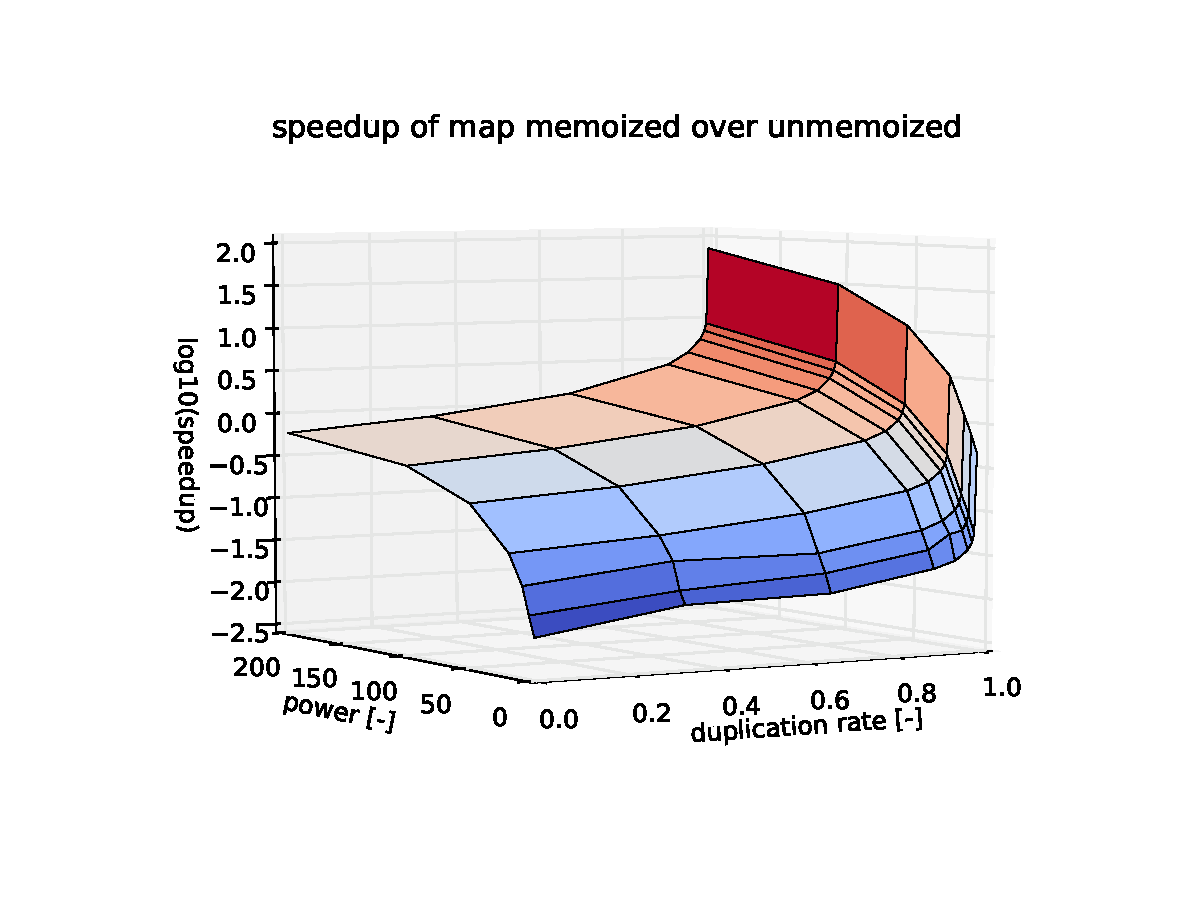
\includegraphics[width=3.50 in, trim=1.00in 1.00in 1.00in .70in, clip]{figures/Main3_mapMemoized_vs_unMemoized_shuffler}}
\hfill
    \subfloat[map-memoized vs un-memoized]{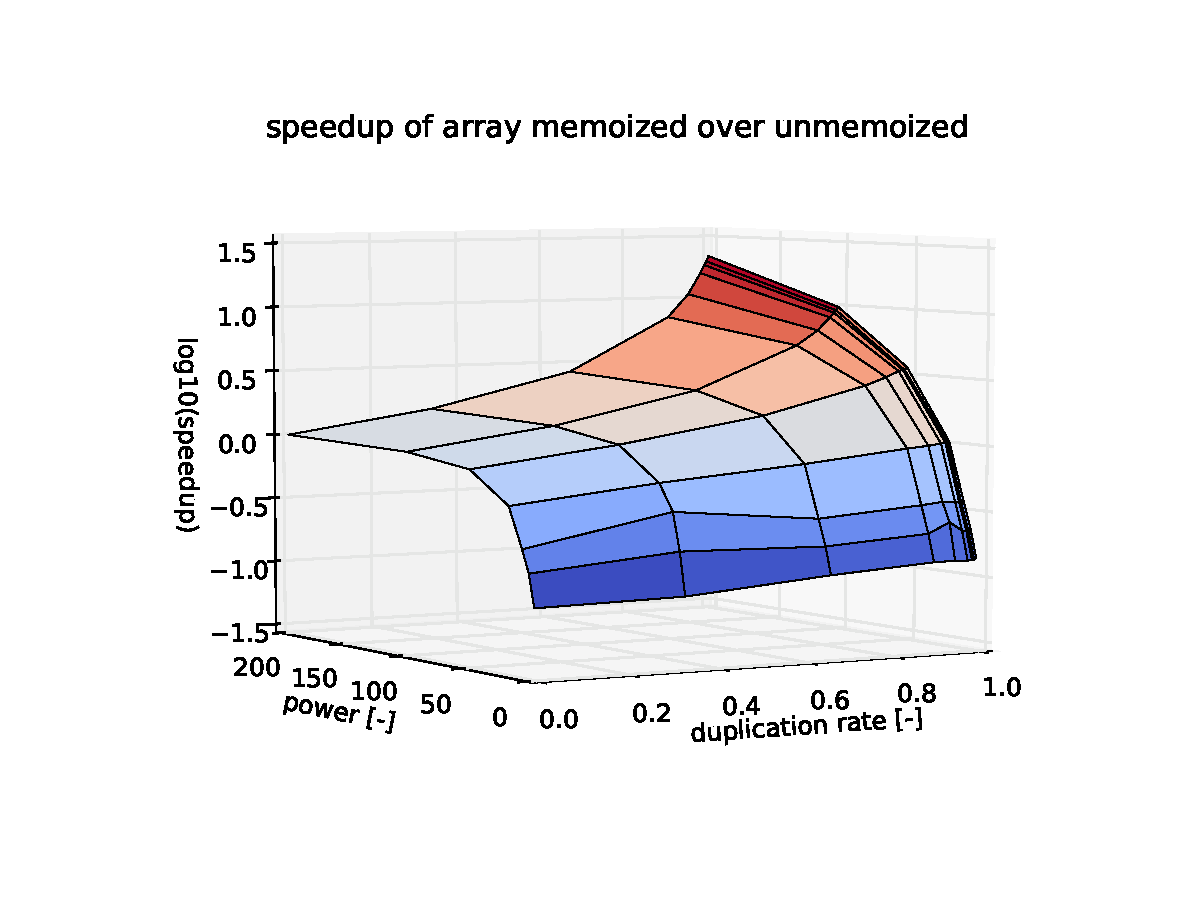
\includegraphics[width=3.50 in, trim=1.00in 1.00in 1.00in .70in, clip]{figures/Main3_arrayMemoized_vs_unMemoized_shuffler}}
    \caption{\label{fig:ArrayAndMapVsUnMemoized}Performance versus un-memoized}
\end{figure}

\begin{figure}[h!]
    \begin{center}
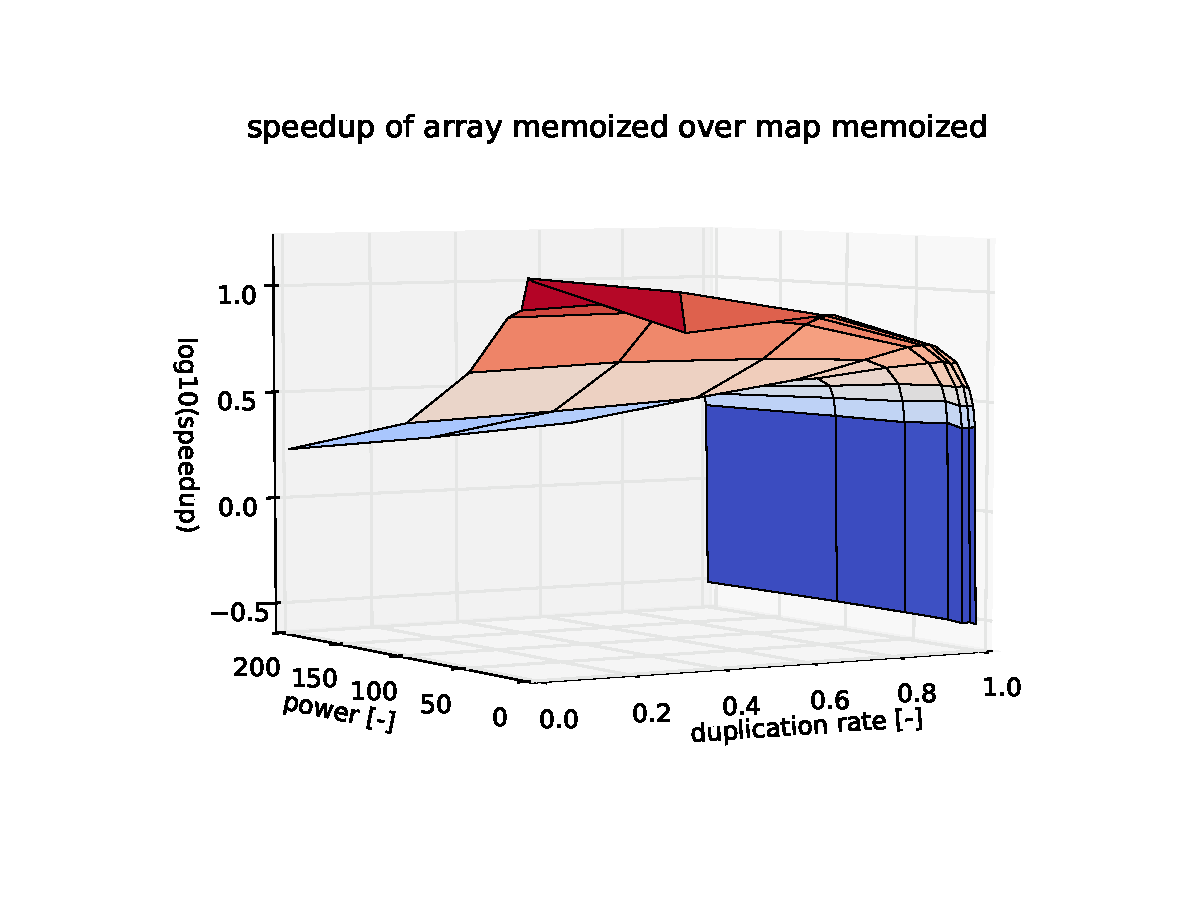
\includegraphics[width=4 in, trim=1.00in 1.00in 1.00in .70in, clip]{figures/Main3_arrayMemoized_vs_mapMemoized_shuffler}
\caption{\label{fig:SpeedupOfArrayMemoizedOverMapMemoized} {Speedup of array-memoized over map-memoized}}
\end{center}
\end{figure}

\fi

In general memoization is not useful unless either the power or the duplication rate are reasonably high, which we expect. However I think this is a pretty unfair comparison because \texttt{std::map} doesn't make sense here. \texttt{std::unordered\_set} or some better hash table should be used instead.

We also learn that array memoization is faster than map memoization in all cases except when duplication rates are very high. This answer seems a little lackluster but I'm not sure what else to add.


\eprob{10}{Back to the Real World}

Provide short (but sufficient) answers to the following prompts:

\begin{enumerate}[a)]
\item Let's say that your tech-y labmate tells you that trying to be smart about programming is dumb because computers get 60\% faster each year, so it's not worth your time.  How would you respond?  What does change by \textasciitilde60\% per year, and what does that have to do with fast programming?  Note: this question is like the next one, but it's to a technical audience.

\ifSolutions

\textbf{Solution:} This 60\% change used to be from clock speed and IPC increases, which basically any serial code would run faster without doing anything. However in the early 2000's when we hit a clock speed ceiling of about 3.5GHz, CPU designers started finding that 60\% by adding vector registers, sepcialized instructions, and more cores. Thus we can't just re-use old serial code, we have to re-write our code to take advantage of this new hardware, which is very diffucult, so it's much harder to actually realize a 60\% real speedup in execution time. To make matters worse, this 60\% speedup is mostly on the CPU side, and memory is not getting much faster. In order to utilize this 60\% increase in CPU performance we have to keep the CPUs fed with data from memory, which means doing increasingly complicated things to better organize our data to be cache-friendly.

\fi

\item Let's say that a ``non-technical'' friend of yours (who knows essentially nothing about computer architecture) talks to you about the good old days in which computers were twice as fast every other year (throwing out a bunch of arcane-sounding model names that end in 86) and asks you ``So, how about now?  How much faster are computers now than they were in 2000?  I bet they're 100 times faster!!1!''  Note: this is like the previous question, but for a non-technical audience.

\ifSolutions

\textbf{Solution:} I'm really having trouble finding a way to explain this one to a non-technical friend.

\fi

\item What is the relationship between the memory footprint of a program, the size of the memory on a machine, the program being memory-bound, and its total runtime?

\ifSolutions

\textbf{Solution:} The memory footprint of a program is the amount of RAM it uses while running. The size of the memory on the machine is the total amount of RAM avalible to the operating system, to be shared by all running programs. If we say a program is memory-bound we usually mean its performance is bound by memory access time, and an increase in CPU speed will not make run any faster. Memory-bound could also mean that the program's memory footprint is larger than the size of the memory on the machine. The total runtime of a program is how long it takes to execute from start to finish. If a program is memory-bound, this runtime can be decreased by making the program more cache-friendly.

\fi

\end{enumerate}

\vfill

\eprob{5}{Feedback}

\begin{enumerate}[a)]
\item How much total time did you spend on this assignment?
\item Of that time, how much total time did you spend ``flailing'' on little annoying things that are not the main point of the assignment?
\item Did you work with anyone closely on this assignment?
\item Did you have any ``aha'' moments where something clicked?  If so, on what problems or parts?
\item Can you give me any other feedback on this assignment?
\end{enumerate}

\vskip 1cm
\total

\end{document}

todo: change the seed of the random number generator to determine student grades at the end.
